\let\negmedspace\undefined
\let\negthickspace\undefined
\documentclass[journal]{IEEEtran}
\usepackage[a5paper, margin=10mm, onecolumn]{geometry}
%\usepackage{lmodern} % Ensure lmodern is loaded for pdflatex
\usepackage{tfrupee} % Include tfrupee package

\setlength{\headheight}{1cm} % Set the height of the header box
\setlength{\headsep}{0mm}     % Set the distance between the header box and the top of the text

\usepackage{gvv-book}
\usepackage{gvv}
\usepackage{cite}
\usepackage{amsmath,amssymb,amsfonts,amsthm}
\usepackage{algorithmic}
\usepackage{graphicx}
\usepackage{textcomp}
\usepackage{xcolor}
\usepackage{txfonts}
\usepackage{listings}
\usepackage{enumitem}
\usepackage{mathtools}
\usepackage{gensymb}
\usepackage{comment}
\usepackage[breaklinks=true]{hyperref}
\usepackage{tkz-euclide} 
\usepackage{listings}
% \usepackage{gvv}                                        
\def\inputGnumericTable{}                                 
\usepackage[latin1]{inputenc}                                
\usepackage{color}                                            
\usepackage{array}                                            
\usepackage{longtable}                                       
\usepackage{calc}                                             
\usepackage{multirow}                                         
\usepackage{hhline}                                           
\usepackage{ifthen}                                           
\usepackage{lscape}

\begin{document}

\bibliographystyle{IEEEtran}
\vspace{3cm}

\title{1-1.2-24}
\author{EE24BTECH11063 - Y.Harsha Vardhan Reddy
}
% \maketitle
% \newpage
% \bigskip
{\let\newpage\relax\maketitle}

\renewcommand{\thefigure}{\theenumi}
\renewcommand{\thetable}{\theenumi}
\setlength{\intextsep}{10pt} % Space between text and floats


\numberwithin{equation}{enumi}
\numberwithin{figure}{enumi}
\renewcommand{\thetable}{\theenumi}
\textbf{Question}:\\
Rain is falling vertically with a speed of $35ms^{-1}$. A woman rides a bicycle with a speed of $12ms^{-1}$ in easty to west direction. What is the direction in which she should hold her umbrella ?
\\
\textbf{Solution: }
\begin{table}[h!]    
  \centering
  \begin{tabular}[12pt]{ |c| c|}
    \hline
    \textbf{Variable} & \textbf{Description}\\ 
    \hline
    $V_1,u_1,f_1$ & Parameters of Parabola \\
    \hline 
    $V_2,u_2,f_2$ & Parameters of circle \\
    \hline
     $P_1,P_2$ & Points of intersection \\
     \hline
     $A$ & Area between the conics \\
    \hline
\end{tabular}

  \caption{Variables Used}
  \label{tab1-1.2-20}
\end{table}
\begin{align}
V_r=\myvec{0\\-35}
\end{align}
\begin{align}
V_w=\myvec{-12\\0}
\end{align}
\begin{align}
V_{rw}=V_r-V_w
\end{align}
\begin{align}
V_{rw}=\myvec{0\\-35}-\myvec{-12\\0}=\myvec{12\\-35}
\end{align}
\begin{align}
    d_w=-V_{rw}
\end{align}
Therefore,
\begin{align}
    d_w=\myvec{-12\\35}
\end{align}
\begin{align}
    \theta = \tan^{-1}\brak{\frac{horizontal component}{vertical component}}
\end{align}
Therefore,
\begin{align}
    \theta = \tan^{-1}\brak{\frac{12}{35}}
\end{align}
\begin{figure}[h!]
   \centering
   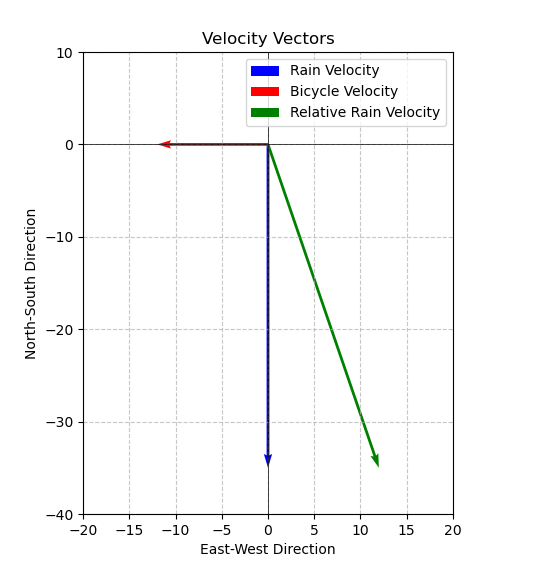
\includegraphics[width=0.7\linewidth]{figure_1.png}
   \label{stemplot}
\end{figure}





\end{document}
